\documentclass[tikz,border=2pt]{standalone}
\usepackage{amsmath,amssymb}
\usepackage{tikz}
\usetikzlibrary{arrows.meta}

\begin{document}
% A bounded set fits inside some interval [-M, M]; its points may be scattered, but none escapes.
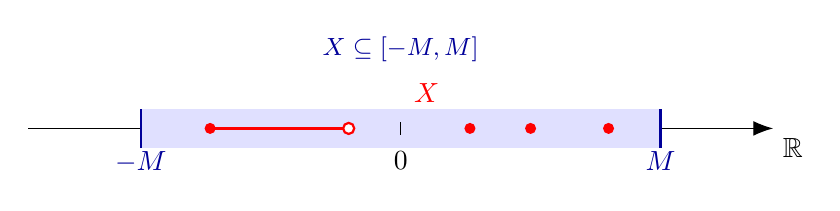
\begin{tikzpicture}[x=1.1cm]
	\draw[-{Latex[length=2.5mm]}] (-4.3,0) -- (4.3,0) node[below right] {$\mathbb{R}$};
	\fill[blue!12] (-3,-0.25) rectangle (3,0.25);
	\draw[blue!60!black, thick] (-3,-0.25) -- (-3,0.25);
	\draw[blue!60!black, thick] (3,-0.25) -- (3,0.25);
	\node[blue!60!black, below=5pt] at (-3,0) {$-M$};
	\node[blue!60!black, below=5pt] at (3,0) {$M$};
	\node[below=5pt] at (0,0) {$0$};
	\draw (0,0.08) -- (0,-0.08);
	% the set X: a segment, a few isolated points
	\draw[very thick, red] (-2.2,0) -- (-0.6,0);
	\fill[red] (-2.2,0) circle (2pt);
	\draw[red, thick, fill=white] (-0.6,0) circle (2pt);
	\fill[red] (0.8,0) circle (2pt);
	\fill[red] (1.5,0) circle (2pt);
	\fill[red] (2.4,0) circle (2pt);
	\node[red, above=6pt] at (0.3,0) {$X$};
	\node[blue!60!black, above=12pt, font=\small] at (0,0.3) {$X\subseteq[-M,M]$};
\end{tikzpicture}
\end{document}
